\chapter{Predicate Logic: Semantics}\label{ch:predsem}

In propositional logic, a valuation (one truth value per atom) is all the meaning we need.
In predicate logic we must say what the objects are and what each symbol denotes.

\section{Interpretations}

\begin{definition}[Interpretation / structure / model]
An \emph{interpretation} $I$ for a language $\mathcal{L}$ consists of
\begin{enumerate}
  \item a non-empty set $D$, the \emph{domain} (universe of discourse);
  \item for each constant symbol $c$, an element $c^I\in D$;
  \item for each $n$-ary function symbol $f$, a function $f^I: D^n\to D$;
  \item for each $n$-ary predicate symbol $P$, a relation $P^I\subseteq D^n$
        (for $n=0$, a truth value).
\end{enumerate}
The equality symbol, if present, is always interpreted as true identity on $D$.
\end{definition}

\begin{important}[Domains are non-empty and functions are total]
The domain must be non-empty, and each $f^I$ must be defined on \emph{all} of $D^n$ with
values in $D$. E.g.\ subtraction is not a valid interpretation of a binary function
symbol on domain $\N$ (since $2-5\notin\N$) unless modified (truncated subtraction).
\end{important}

\section{Environments and evaluation}

Formulas with free variables need values for them.

\begin{definition}[Environment]
An \emph{environment} (variable assignment) for $I$ is a function $E$ from variables to
$D$. For $d\in D$, $E[x\mapsto d]$ is the environment equal to $E$ except it maps $x$
to $d$.
\end{definition}

\begin{definition}[Value of a term]
\[x^{(I,E)} = E(x),\qquad c^{(I,E)}=c^I,\qquad
f(t_1,\dots,t_n)^{(I,E)} = f^I\big(t_1^{(I,E)},\dots,t_n^{(I,E)}\big).\]
\end{definition}

\begin{definition}[Satisfaction]
We define $I\models_E\varphi$ (\emph{$I$ satisfies $\varphi$ under $E$}) recursively:
\begin{itemize}
  \item $I\models_E P(t_1,\dots,t_n)$ iff $\big(t_1^{(I,E)},\dots,t_n^{(I,E)}\big)\in P^I$;
  \item $I\models_E t_1=t_2$ iff $t_1^{(I,E)} = t_2^{(I,E)}$;
  \item connectives as in propositional logic, e.g.\ $I\models_E\neg\varphi$ iff
        $I\not\models_E\varphi$, and $I\models_E \varphi\to\psi$ iff $I\not\models_E\varphi$
        or $I\models_E\psi$;
  \item $I\models_E\forall x\,\varphi$ iff $I\models_{E[x\mapsto d]}\varphi$ for
        \emph{every} $d\in D$;
  \item $I\models_E\exists x\,\varphi$ iff $I\models_{E[x\mapsto d]}\varphi$ for
        \emph{some} $d\in D$.
\end{itemize}
\end{definition}

\begin{lemma}
Whether $I\models_E\varphi$ depends only on $E$'s values on $FV(\varphi)$. In particular,
for a sentence $\varphi$ the environment is irrelevant and we write $I\models\varphi$
(``$\varphi$ is true in $I$'', ``$I$ is a model of $\varphi$'').
\end{lemma}

\begin{example}
Language: binary predicate $R$, constant $c$. Let $\varphi=\forall x\,\exists y\,R(x,y)$
and $\psi = \exists y\,\forall x\,R(x,y)$.
\begin{itemize}
  \item $I_1$: $D=\N$, $R^{I_1}= {<}$. Then $I_1\models\varphi$ (for each $n$ take $n+1$)
        but $I_1\not\models\psi$ (no largest natural number).
  \item $I_2$: $D=\N$, $R^{I_2}={\ge}$. Then $I_2\models\psi$ (take $y=0$, since $x\ge0$
        for all $x$), so also $I_2\models\varphi$.
  \item $I_3$: $D=\{1,2\}$, $R^{I_3}=\{(1,2)\}$. Then $I_3\not\models\varphi$ since $2$
        is not related to anything.
\end{itemize}
Small interpretations are easy to draw: elements as dots, a binary relation as arrows.
\begin{center}
\begin{tikzpicture}[>=Stealth,p/.style={circle,fill=blue!50!black,inner sep=2pt}]
  \draw[rounded corners,gray] (-0.7,-0.7) rectangle (3.1,0.8);
  \node[font=\scriptsize,gray,anchor=north west] at (-0.7,0.8) {$D$};
  \node[p,label=below:{\small $1$}] (a) at (0,0) {};
  \node[p,label=below:{\small $2$}] (b) at (2.4,0) {};
  \draw[->,thick] (a) -- node[above,font=\scriptsize]{$R$} (b);
  \node[font=\scriptsize,red!70!black,anchor=west] at (3.3,0) {no arrow leaves $2$, so $\forall x\,\exists y\,R(x,y)$ fails};
\end{tikzpicture}
\end{center}
\end{example}

\begin{example}[Evaluating with an environment]
$I$: $D=\Z$, $f^I(a,b)=a+b$, $c^I=0$, $P^I = \{(a,b): a<b\}$. Let
$\varphi = \exists y\,P(f(x,y),c)$ and $E(x)=5$. We need some $d\in\Z$ with $5+d<0$;
$d=-6$ works, so $I\models_E\varphi$. In fact $I\models_E\varphi$ for every $E$, so
$I\models\forall x\,\varphi$.
\end{example}

\section{Validity, satisfiability, consequence}

\begin{definition}
\begin{itemize}
  \item $\varphi$ is \emph{satisfiable} if $I\models_E\varphi$ for some $I$ and $E$.
  \item $\varphi$ is \emph{valid} (logically true), written $\models\varphi$, if
        $I\models_E\varphi$ for every $I$ and $E$.
  \item A set $\Sigma$ is satisfiable if some single $(I,E)$ satisfies every formula
        in $\Sigma$.
  \item $\Sigma\models\varphi$ (\emph{$\varphi$ is a logical consequence of $\Sigma$}) if
        every $(I,E)$ that satisfies all of $\Sigma$ also satisfies $\varphi$.
  \item $\varphi\equiv\psi$ if $\varphi\models\psi$ and $\psi\models\varphi$.
\end{itemize}
\end{definition}

\begin{center}
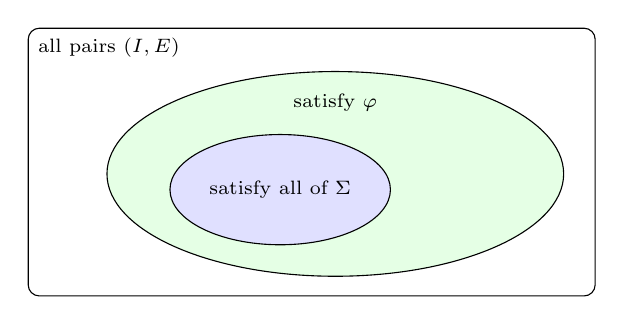
\begin{tikzpicture}[font=\small]
  \draw[rounded corners] (-3.6,-1.7) rectangle (3.6,1.7);
  \node[anchor=north west,font=\scriptsize] at (-3.6,1.7) {all pairs $(I,E)$};
  \draw[fill=green!10] (0.3,-0.15) ellipse (2.9cm and 1.3cm);
  \draw[fill=blue!12] (-0.4,-0.35) ellipse (1.4cm and 0.7cm);
  \node[font=\scriptsize] at (-0.4,-0.35) {satisfy all of $\Sigma$};
  \node[font=\scriptsize] at (0.3,0.75) {satisfy $\varphi$};
\end{tikzpicture}

\small $\Sigma\models\varphi$: every model of $\Sigma$ is a model of $\varphi$. $\varphi$ is valid when its
region is the whole rectangle, and satisfiable when its region is non-empty.
\end{center}

The same facts as before hold: $\Sigma\models\varphi$ iff $\Sigma\cup\{\neg\varphi\}$ is
unsatisfiable, and $\Sigma\cup\{\varphi\}\models\psi$ iff $\Sigma\models\varphi\to\psi$
(for sentences $\varphi$).

\begin{important}[How to prove/disprove semantic claims]
\begin{itemize}
  \item To show $\Sigma\not\models\varphi$ (or that $\varphi$ is not valid): give a
        \emph{specific} interpretation (domain + meaning of every symbol) making all of
        $\Sigma$ true and $\varphi$ false. Small finite domains are often easiest.
  \item To show $\Sigma\models\varphi$: take an \emph{arbitrary} interpretation $I$ and
        environment $E$ satisfying $\Sigma$, and reason from the definition of
        satisfaction that $I\models_E\varphi$.
\end{itemize}
\end{important}

\begin{example}[Proving a consequence]
Show $\forall x\,(P(x)\to Q(x)),\ \forall x\,P(x)\models\forall x\,Q(x)$.

Let $(I,E)$ satisfy both premises and let $d\in D$ be arbitrary. By the second premise,
$d\in P^I$. By the first, with $x\mapsto d$, if $d\in P^I$ then $d\in Q^I$. So $d\in Q^I$.
Since $d$ was arbitrary, $I\models_E\forall x\,Q(x)$.
\end{example}

\begin{example}[Disproving a consequence]
Show $\forall x\,(P(x)\lor Q(x))\not\models\forall x\,P(x)\lor\forall x\,Q(x)$.

Take $D=\{1,2\}$, $P^I=\{1\}$, $Q^I=\{2\}$. Every element is in $P^I$ or $Q^I$, so the
premise holds; but neither $P^I$ nor $Q^I$ is all of $D$, so the conclusion fails.
\begin{center}
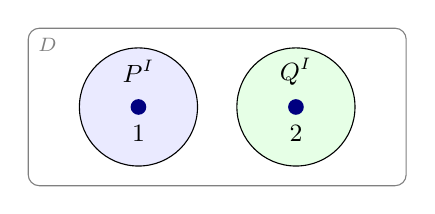
\begin{tikzpicture}[p/.style={circle,fill=blue!50!black,inner sep=2pt}]
  \draw[rounded corners,gray] (-1.4,-1) rectangle (3.4,1);
  \node[font=\scriptsize,gray,anchor=north west] at (-1.4,1) {$D$};
  \draw[fill=blue!10,fill opacity=0.8] (0,0) circle (0.75cm);
  \draw[fill=green!12,fill opacity=0.8] (2,0) circle (0.75cm);
  \node[p,label=below:{\small $1$}] at (0,0) {};
  \node[p,label=below:{\small $2$}] at (2,0) {};
  \node[font=\small] at (0,0.45) {$P^I$};
  \node[font=\small] at (2,0.45) {$Q^I$};
\end{tikzpicture}
\end{center}
\end{example}

\begin{example}
$\exists x\,\forall y\,R(x,y)\models\forall y\,\exists x\,R(x,y)$ is valid: if $d_0$ is
related to everything, then for each $e$ we can pick $x=d_0$. The converse fails:
interpret $R$ as equality on a two-element domain. Everything equals something, but
nothing equals everything.
\end{example}

\section{Important equivalences}

\begin{important}[Quantifier laws]
\begin{tabular}{@{}ll@{}}
Negation (De Morgan) & $\neg\forall x\,\varphi\equiv\exists x\,\neg\varphi$,\quad
  $\neg\exists x\,\varphi\equiv\forall x\,\neg\varphi$\\
Distribution & $\forall x\,(\varphi\land\psi)\equiv\forall x\,\varphi\land\forall x\,\psi$\\
 & $\exists x\,(\varphi\lor\psi)\equiv\exists x\,\varphi\lor\exists x\,\psi$\\
Commutation & $\forall x\,\forall y\,\varphi\equiv\forall y\,\forall x\,\varphi$,\quad
  $\exists x\,\exists y\,\varphi\equiv\exists y\,\exists x\,\varphi$\\
\multicolumn{2}{@{}l}{If $x\notin FV(\psi)$:}\\
 & $\forall x\,\varphi\land\psi\equiv\forall x\,(\varphi\land\psi)$,\quad
   $\exists x\,\varphi\lor\psi\equiv\exists x\,(\varphi\lor\psi)$\\
 & $\forall x\,\varphi\lor\psi\equiv\forall x\,(\varphi\lor\psi)$,\quad
   $\exists x\,\varphi\land\psi\equiv\exists x\,(\varphi\land\psi)$\\
 & $\psi\to\forall x\,\varphi\equiv\forall x\,(\psi\to\varphi)$,\quad
   $\psi\to\exists x\,\varphi\equiv\exists x\,(\psi\to\varphi)$\\
 & $(\forall x\,\varphi)\to\psi\equiv\exists x\,(\varphi\to\psi)$,\quad
   $(\exists x\,\varphi)\to\psi\equiv\forall x\,(\varphi\to\psi)$
\end{tabular}
\end{important}

Note the flip in the last line: a quantifier in the antecedent of $\to$ changes type when
pulled out. Also note the \emph{non}-equivalences:
$\forall x\,(\varphi\lor\psi)\not\equiv\forall x\,\varphi\lor\forall x\,\psi$ and
$\exists x\,(\varphi\land\psi)\not\equiv\exists x\,\varphi\land\exists x\,\psi$
(only $\models$ in one direction).

\begin{aside}
Using these laws (and renaming bound variables), every formula can be converted to
\emph{prenex normal form}: a string of quantifiers followed by a quantifier-free matrix,
e.g.\ $\forall x\,\exists y\,\forall z\,(\dots)$. Prenex form plus \emph{Skolemisation}
(replacing $\exists y$ inside $\forall x$ by a new function $f(x)$) and CNF conversion is
how resolution is extended to first-order logic, together with \emph{unification} of terms.
\end{aside}

\section{Theories and models}

A set of sentences $\Sigma$ often serves as axioms describing a class of structures.

\begin{example}[Partial orders]
Language: binary predicate $\le$. Axioms:
\begin{align*}
&\forall x\,(x\le x), \quad
 \forall x\,\forall y\,(x\le y\land y\le x\to x=y),\\
&\forall x\,\forall y\,\forall z\,(x\le y\land y\le z\to x\le z).
\end{align*}
Models include $(\N,\le)$, $(\mathcal{P}(S),\subseteq)$ and $(\Z^+,\mid)$. Adding
$\forall x\,\forall y\,(x\le y\lor y\le x)$ excludes $\subseteq$ and $\mid$.
Hasse diagrams of two of these models (an edge going up means ``$\le$''):
\begin{center}
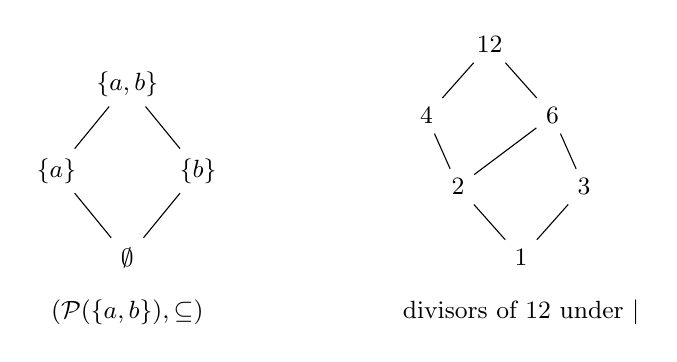
\begin{tikzpicture}[font=\small]
  \node (e) at (0,0) {$\emptyset$};
  \node (a) at (-0.9,1.1) {$\{a\}$};
  \node (b) at (0.9,1.1) {$\{b\}$};
  \node (ab) at (0,2.2) {$\{a,b\}$};
  \draw (e) -- (a) -- (ab) -- (b) -- (e);
  \node at (0,-0.7) {$(\mathcal{P}(\{a,b\}),\subseteq)$};
  \begin{scope}[xshift=5cm]
  \node (1) at (0,0) {$1$};
  \node (2) at (-0.8,0.9) {$2$};
  \node (3) at (0.8,0.9) {$3$};
  \node (4) at (-1.2,1.8) {$4$};
  \node (6) at (0.4,1.8) {$6$};
  \node (12) at (-0.4,2.7) {$12$};
  \draw (1) -- (2) -- (4) -- (12) -- (6) -- (3) -- (1);
  \draw (2) -- (6);
  \node at (0,-0.7) {divisors of $12$ under $\mid$};
  \end{scope}
\end{tikzpicture}

\small Neither is a total order: $\{a\}$ and $\{b\}$ are incomparable, as are $4$ and $6$.
\end{center}
\end{example}

\begin{example}[Expressing size]
$\exists x\,\exists y\,\neg(x=y)$ is true exactly in interpretations with at least two
elements. $\forall x\,\forall y\,(x=y)$ holds exactly when $|D|=1$. With these one can
express ``at least $n$'' and ``at most $n$'' for each fixed $n$, but (by compactness)
no set of sentences is true in exactly the finite interpretations.
\end{example}

\section*{Summary}
\begin{itemize}
  \item An interpretation gives a non-empty domain and meanings for constants, functions
        (total) and predicates; an environment gives values to variables.
  \item $\forall x\,\varphi$ is true iff $\varphi$ holds for every value of $x$; $\exists$
        iff for some value.
  \item Valid: true in every $(I,E)$; satisfiable: true in some; $\Sigma\models\varphi$:
        every model of $\Sigma$ is a model of $\varphi$.
  \item Disprove with a concrete counter-interpretation; prove by reasoning about an
        arbitrary one.
  \item Quantifier laws: De Morgan, distribution of $\forall$ over $\land$ and $\exists$
        over $\lor$, pulling quantifiers past formulas without the variable free.
\end{itemize}
